\documentclass[10pt, conference, compsocconf]{IEEEtran}

\usepackage[ruled,linesnumbered,lined,commentsnumbered]{algorithm2e}
\SetAlFnt{\small}
\SetAlCapFnt{\small}
\SetAlCapNameFnt{\small}
\usepackage{algorithmic}
\algsetup{linenosize=\tiny}
\usepackage[tight]{subfigure}
\usepackage{graphicx}
\usepackage{multicol,lipsum}
\usepackage{amsfonts}
\usepackage{booktabs}
\usepackage{siunitx}
\usepackage{mathtools}
\usepackage{breqn}
\usepackage{placeins}
\usepackage{balance}


%
\ifCLASSINFOpdf
\else
\fi
\hyphenation{op-tical net-works semi-conduc-tor}

\SetKwRepeat{Do}{do}{while}


\begin{document}
\title{StreamNet: Enabling Large Scale DAG based Nakamoto Consensus through Streaming Graph Computing}

\maketitle




\begin{abstract}
%TRIAS StreamNet is a DAG (Directed Asyclyc Graph) blockchain design rooted from the existing mature systems. 
Considering major issues in the existing DAG systems such as centralization caused by the introduction of Coordinator, double-spending and sybil attacks, slow transaction speed etc. 
We designed and implemented the StreamNet system which is forked from the IOTA implementation.
By leveraging the Topological sorting and Katz centrality computation, we infer a pivotal chain along the path of each topological level in the graph,
and each block in the pivotal chain will have the highest Katz centrality score, which could be used as the entry point for the tip selection algorithm.
In addtion, with comprehensive integration of information such as transaction (vertices), 
transaction approval information (edges), and network structure (such as community structure) we designed the tip selection algorithm that obeys the local modifier method and can detect and avoid double spend / sybil attacks.


\end{abstract}

\begin{IEEEkeywords}
Block chain, DAG

\end{IEEEkeywords}


\IEEEpeerreviewmaketitle



% no \IEEEPARstart
\section{Introduction}
Ever since bitcoin \cite{nakamoto2008bitcoin} has been proposed, blockchain technology has been widely studied for $10$ years. 
Extensive adoptions of blockchain technologies was seen in real world applications such as 
financial services with potential regulation challenges \cite{michael2018blockchain, tapscott2017blockchain}, 
supply chains \cite{korpela2017digital,tian2016agri, abeyratne2016blockchain}, 
health cares \cite{azaria2016medrec,yue2016healthcare} and IOT devices \cite{christidis2016blockchains}.
The core of blockchain technology depends on the consensus algorihtms applying to the open distrubuted computing world.
Where computers can join and leave the network and these copmuters can cheat.

As the first protocol that can solve the so called Byzantine general's problem, 
bitcoin system suffers from the problem of low transaction rate with a transaction per second (TPS) of approximately $7$, and long confirmation time (about an hour).
As more and more machines joined the network, they are competing for the privileges to attach the block (miners) which result in huge waste of electric power.
While sky rocketing fees are payed to make sure the transfers of money will be placed in the chain.
On par, there are multiple proposals to solve the low transaction speed issue. 

One method intends to solve the speed problem without changing the chain data structure, for instance, 
the bitcoin cash (BCH) fork of bitcoin (BTC) system tries to improve the throughput of the system by enlarging the data size of each block from $1$ Mb to $4$ Mb. 
To minimize the cost of POW, a proof of stake method POS \cite{wood2014ethereum} is proposed to make sure that only those who in the network have the privilege to attach the block only if they have a large amount of token shares.
Anohter idea targeting at utilizing the power in POW to do useful and meaningful tasks such as training machine learning models are also proposed \cite{matthew2017aion}.
In addition, inspired by the PBFT algorithm \cite{castro1999practical} and a set of its relateted variations, so called hybrid (or consortium) chain was proposed. 
The general idea is to use two step algorithm, the first step is to elect a commiette, the second step is collecting committee power to employ PBFT for consensus.
Bitcoin-NG \cite{eyal2016bitcoin} is the early adoptor of this idea, which splits the blocks of bitcoin into two groups, one is for master election and another for regular transaction blocks. 
Honey-badger \cite{miller2016honey} is the system that firstly introducted the consensus commitee, it uses a predefined memebers to perform PBFT algorithm to reach consensus.  
The Byzcoin system \cite{kogias2016enhancing} brought forth the idea of POW for the commitee election, and uses a variation of PBFT called collective signing for speed purposes.
The Algorand \cite{gilad2017algorand} utilizes a random function to anonymously elect commetee and use this commitee to commit blocks, and the member of the commitee only have one chance to commit block.
All these systems have one common feature, the split of layers of players in the network, which results in the complexity of the implementation of the system.

While aforemetioned methods are trying to avoid side chains, another thread of effort is put on using direct acyclic graph DAG to merge side chains.
The first ever idea comes with growing the blockchain with trees instead of chains \cite{sompolinsky2013accelerating}, which results in the well known GHOST protocol \cite{sompolinsky2015secure}.
If one block links to $\geq 2$ previous blocks, then the data structure grows like a DAG instead of tree \cite{sompolinsky2016spectre, sompolinskyphantom, lewenberg2015inclusive}.
There is a improvement of the GHOST based DAG algorithm which can achieve $6000$ of TPS in reality \cite{li2018scaling}.
Another set of methods tried to avoid finality of constructing a linear total order by introducing the probability of confirmation in the network \cite{popov2016tangle, churyumov2016byteball}. 
However, suffering from engineering issues, mainly due to the lack of transaction frquency and the growing complexity due to the network expansion.
These system in reality are rely on centralized mehods to maintain their stability.
Some of the side chain methods also borrows the idea of DAG, such as nano \cite{lemahieu2018nano} and vite \cite{liuvite}.

%All of the current DAG systems used the idea of head counting method to infer main chains which does not consider the network structure.
%Dating back to the time Google uses PageRank \cite{page1999pagerank} to sort importance of web page instead of number of references, and this method has achieved a huge susccess.
%And this method can also be utilized to help growing the DAG, in this paper, we use the Katz centrality metric \cite{katz1953new}.
Emerging social network research has introduced the method of streaming graph analysis \cite{ediger2011tracking, green2012fast, ediger2012stinger} which deals
with how to quickly maintain information on a temporally or spatially changing graph without traversing the whole graph. 
We view the DAG based method as a streaming graph problem which is about how to compute the total order and achieve consensus without consuming more computing power.
The main contribution of this paper is how to utilize the streaming graph analysis methods to bring the DAG systems into real decentralized, and stabilized growing system.


\section{Basic design}


\subsection{Data structure}

The local state of a node in the StreamNet protocol is a direct acyclic graph (DAG) $G = <B,g,P,E>$. 
$B$ is the set of blocks in $G$. 
$g \in G$ is the genesis block. 
For instance, vertex $g$ in Figure~\ref{simple_sn} represents the Genesis block.
$P$ is a function that maps a block $b$ to its parent block $P(b)$. Specially, $P(g) = \perp$. 
In Figure~\ref{simple_sn}, parent relationships are denoted by solid edges.
Note that there is always a parent edge from a block to its parent block (i.e., $\forall b \in B$, $b, P(b)> \in E$). 
$E$ is the set of directly reference edges and parent edges in this graph. 
$e = <b,b'> \in E$ is an edge from the block $b$ to the block $b'$, 
which means that $b'$ happens before $b$. 
For example in Figure~\ref{simple_sn}, vertex $1$ represents the first block, which is the parent for the subsequent block $2$, $3$ and $4$. 
Vertex $5$ has two edges, one is the parent edge pointing to $3$, another is reference edge pointing to $4$.
When a new block is not referenced, it is called a tip. For example, in Figure~\ref{simple_sn}, block $6$ is a tip.
All blocks in the StreamNet protocol share a predefined deterministic 
hash function Hash that maps each block in $B$ to a unique integer id . 
It satisfies that $\forall {b} \neq {b'}$, Hash($b$) $\neq$ Hash($b'$).

\begin{figure}[!ht]
\begin{center}
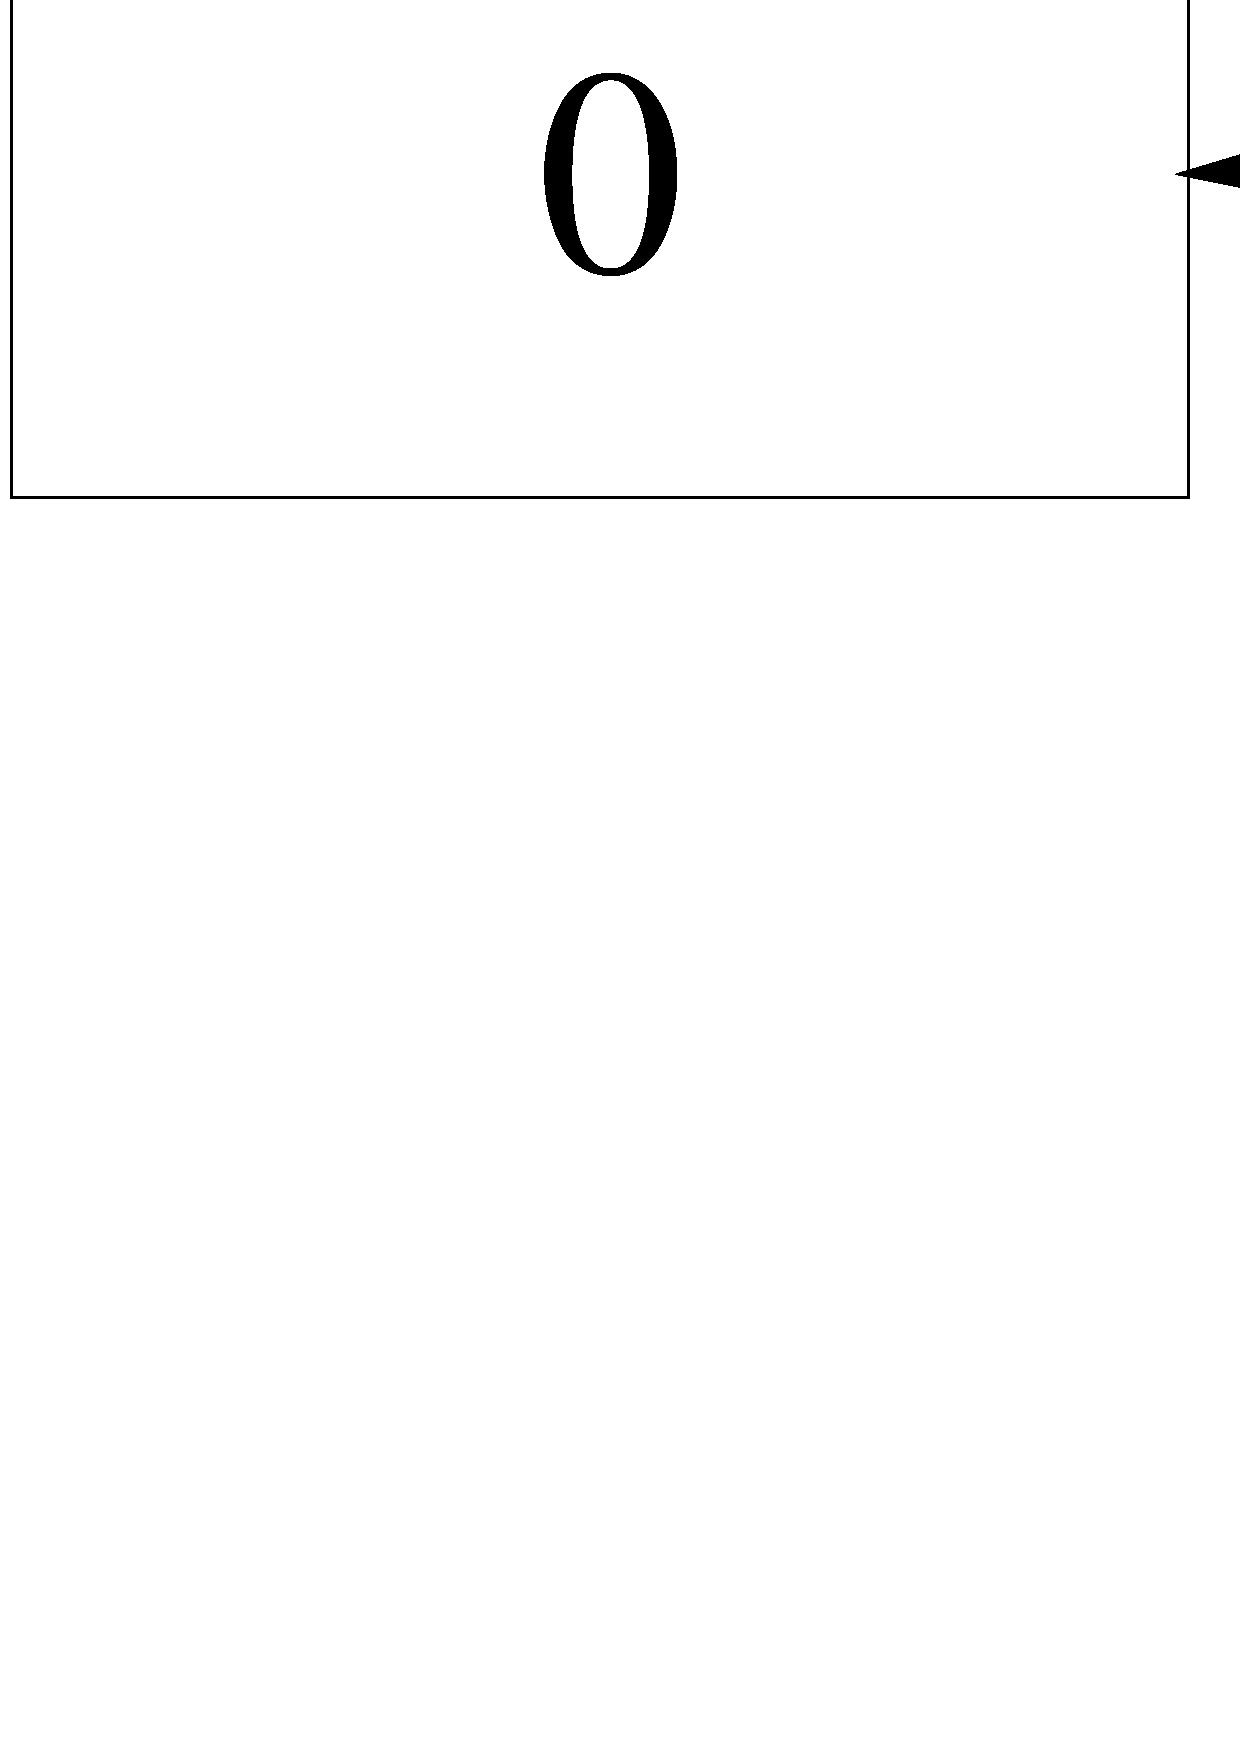
\includegraphics[width=0.45\textwidth]{figures/simple_sn.pdf}
    \caption{
        Example of the StreamNet data structure.
     }
\label{simple_sn}
\end{center}
\end{figure}

\subsection{StreamNet Architecture}

Figure~\ref{architecture} presents the architecture of StreamNet,
it's consists of multiple StreamNet machines.
Each StreamNet machine will grow its DAG locally, and will broadcast the changes using gossip protocol. 
Eventually, every machine will have a unified view of DAG.
By calling total ordering algorithm, every machine can sort the DAG into a total order, 
and the data in each block can have a relative order regardless of their local upload time.
Figure~\ref{node} shows the local architecture of StreamNet.
In each StreamNet node, there will be a transaction pool accepting the transactions from the HTTP API.
And there will be a block generator to pack a certain amount of transactions into a block, it firstly find a 
parent and reference block to attach the new block to, based on the hash information of these two blocks and the meta data of the block itself, 
it will then perform the proof of work (POW) to calculate the nonce for the new block.
Algorithm~\ref{algo:main_loop} summarize the server logic for a StreamNet node.
In the algorithm, the way to find parent block is by $Pivot(G, g)$.
And the way to find reference block is by calling $MCMC(G, g)$ which is the Markov Chain Monte Carlo (MCMC) random walk algorithm \cite{popov2016tangle}.
The two algorithms will be described in the later section.

\begin{figure}[!ht]
\begin{center}
\includegraphics[width=0.45\textwidth]{figures/architecture.pdf}
    \caption{
        StreamNet architecture.
     }
\label{architecture}
\end{center}
\end{figure}

\begin{figure}[!ht]
\begin{center}
\includegraphics[width=0.45\textwidth]{figures/node.pdf}
    \caption{
        One node in StreamNet protocol.
     }
\label{node}
\end{center}
\end{figure}

\IncMargin{1em}
\begin{algorithm}
\SetKwData{Left}{left}\SetKwData{This}{this}\SetKwData{Up}{up}
\SetKwFunction{Union}{Union}\SetKwFunction{FindCompress}{FindCompress}
\SetKwInOut{Input}{input}\SetKwInOut{Output}{output}

\KwIn{ Graph $G=<B, g, P, E>$ }

    \While {Node is running}{
        \uIf{Received $G' = <B', g, P', E'> $}{
            $G'' \gets <B \cup B', g, P \cup P', E \cup E' > $\;
            \uIf{$G \neq G''$ } {
                $G \gets G''$ \;
                Broadcase updated G to neighbors \;
            }
        } 

        \uIf{Generate block $b$}{
            $a \gets Pivot(G, g) $ \;
            $r \gets MCMC(G, g) $ \;
            $G \gets <B \cup b, g, P \cup <b, a>, E \cup <b, a> \cup <b, r> >$ \;
            Broadcase updated G to neighbors \;
        } 
    }

\caption{{ StreamNet node main loop.}}
\label{algo:main_loop}
\end{algorithm}
\DecMargin{1em}


\IncMargin{1em}
\begin{algorithm}
\SetKwData{Left}{left}\SetKwData{This}{this}\SetKwData{Up}{up}
\SetKwFunction{Union}{Union}\SetKwFunction{FindCompress}{FindCompress}
\SetKwInOut{Input}{input}\SetKwInOut{Output}{output}

\KwIn{ The local state $G$ = $<B,g,P,E>$  and a starting block $b \in B$ }
\KwOut{ A random tip $t$ }

$t \leftarrow b$

\Do { Score(G,t) != 0} {
    \For {$b' \in Child(G,t)$} {
        $P_{bb'} = \frac{e^{\alpha Score(G,b')}}{\Sigma_{z:z \rightarrow b}e^{\alpha Score(G,z)}}$
    }
    $t \leftarrow $ choose $b''$ by $P_{bb''}$
}

\Return{$t$} \;

\caption{{\sc MCMC($G$, $b$).}}
\label{algo:mcmc}
\end{algorithm}
\DecMargin{1em}



\subsection{Consensus protocol}
Based on predefined data structure, to present the StreamNet consensus algorithm, 
we firstly define several utility functions and notations, which is a variation from the definition in the Conflux paper \cite{li2018scaling}. 
Chain() returns the chain from the genesis block to a given block following only parent edges. 
$\overline{Chain(G,b)}$ returns all blocks except those in the chain.
Child() returns the set of child blocks of a given block. 
Sibling() returns the set of siblings of a given block. 
Subtree() returns the sub-tree of a given block in the parental tree. 
Before() returns the set of blocks that are immediately generated before a given block. 
Past() returns the set of blocks that are generated before a given block (but including the block itself).
After() returns the set of blocks that are immediately generated after a given block. 
Later() returns the set of blocks that are generated after a given block (but including the block itself).
SubGraph() returns the sub graph by removing blocks and edges except the initial set of blocks.
ParentScore() presents the weight of blocks, each block have a score when referenced as parent. 
Score() presents the weight of blocks, each block achieves a score when attaching to the graph. 
TotalOrder() returns the `flatten' order inferred from the consensus algorithm.
Figure~\ref{allMethods} represents the definition of these utility functions. 

\begin{figure}
\begin{flalign*}
  &\fbox{G = $<B,g,P,E>$} \\
  &Chain(G,b) =
  \begin{cases}
    g                 & \text{b = g} \\
    Chain(G,P(b))     & \text{otherwise}
  \end{cases} \\
  & \overline{Chain(G,b)} = \{ b' | b' \in B, b' \notin Chain(G,b) \} \\
   &Child(G,b) = \{ b'| P(b') = b \} \\
   &Sibling(G,b) = Child(G,P(b)) \\
   &SubTree(G,b) = (U_{i\in Child(G,b)}Substree(G,i)) \cup \{b\} \\
   &Before(G,b) = \{b'|b' \in B, <b,b'> \in E \} \\
   &Past(G,b) = (U_{i\in Before(G,b)}Past(G,i)) \cup \{b\} \\
   &After(G,b) = \{b'|b' \in B, <b',b> \in E \} \\
   &Later(G,b) = (U_{i\in After(G,b)}Later(G,i)) \cup \{b\} \\
   &SubGraph(G,B') = <B', P', E'> | \\
   & \forall <b, b'> \in E', b \subset B' \& b' \subset B'\\
   &ParentScore(G,b) = |SubTree(G,b)| \\
   &Score(G,b) = |Later(G,b)| \\
   &TotalOrder(G) = StreamNetOrder(G,Pivot(G,g)) 
\end{flalign*}

    \caption{The Definitions of Chain(), Child(), Sibling(), Subtree(), Before(), Past(), After(), Later(), SubGraph(), ParentScore(), Score(), and TotalOrder(). }
\label{allMethods}
\end{figure}

\subsubsection{Parent tip Selection by pivotal chain} 
The algorithm Algorithm~\ref{algo:getPivot} presents our pivot chain selection algorithm(i.e., the definition of $Pivot(G, b)$). 
Given a StreamNet state $G$, Pivot($G$,$g$) returns the last block in the pivot chain starting from the genesis block $g$. 
The algorithm recursively advances to the child block whose corresponding sub-tree has the largest number of children. 
Which is calculated by $ParentScore(G, b)$  
When there are multiple child blocks with the same score, the algorithm selects the child block with the largest block hash. 
The algorithm terminates until it reaches a tip. 
Each block in the pivot chain defines a epoch in the DAG, the nodes in DAG that satisfy Past($G$,$b$) - Past($G$,$p$) will belong to the epoch of block $b$.
For example, in Figure~\ref{total_order}, the pivot chain is $<g, 1, 3, 5, 6>$, and the epoch of block $5$ contains two blocks $4$ and $5$.

\IncMargin{1em}
\begin{algorithm}
\SetKwData{Left}{left}\SetKwData{This}{this}\SetKwData{Up}{up}
\SetKwFunction{Union}{Union}\SetKwFunction{FindCompress}{FindCompress}
\SetKwInOut{Input}{input}\SetKwInOut{Output}{output}

\KwIn{ The local state $G$ = $<B,g,P,E>$  and a starting block $b \in B$ }
\KwOut{ The tip in the pivot chain }

\Do { Child(G,b) != 0} {
  $b'$ $\gets$ Child($G,b$)  \;
  $tmpMaxScore$ $\gets$ -1 \;
  $tmpBlock$ $\gets$ $\perp$ \;
  \For {$b' \in Child(G,b)$} {
    $pScore$ $\gets$ ParentScore($G, b'$) \;
    \If { $score$ $>$ $tmpMaxScore$ $||$ ($score$ = $tmpMaxScore$ \text{and Hash($b'$ ) $<$ Hash($tmpBlock$)}} {
      $tmpMaxScore$ $\gets$ $pScore$ \;
      $tmpBlock$ $\gets$ $b'$ \; 
    }
  }
  $b$ $\gets$ $tmpBlock$ \;
}

\Return{$b$} \;

\caption{{\sc pivot($G$, $b$).}}
\label{algo:getPivot}
\end{algorithm}
\DecMargin{1em}



\subsubsection{Reference tip selection by MCMC} 

The tip selection method by using Monte Carlo Random Walk (MCMC) is as Algorithm~\ref{algo:mcmc} shows.
Starting from the genesis, each random walk step will choose a child to jump to,
and the probability of jumping from one block to the next block will be calculated using the formula in the algorithm.
$\alpha$ in the formula is an constant that is used to scale the randomness of the MCMC function, the smaller it is, the more randomness will be in the MCMC function.
The algorithm returns until it finds a tip.

\subsubsection{Total Order} 
The algorithm Algorithm~\ref{algo:conflux_order} defines StreamNetOrder(), 
which corresponds to our block ordering algorithm. 
Given the local state $G$ and a block $b$ in the pivot chain, 
StreamNetOrder($G$, $b$) returns the ordered list of all blocks that appear in or before the epoch of $b$. 
Using StreamNetOrder(), the total order of a local state $G$ is defined as TotalOrder($G$). 
The algorithm recursively orders all blocks in previous epochs(i.e., the epoch of $P(b)$ and before). 
It then computes all blocks in the epoch of $b$ as $B_\Delta$. 
It topologically sorts all blocks in $B_\Delta$ and appends it into the result list. 
The algorithm utilizes the unique hash to break ties. 
In Figure~\ref{total_order}, the final total order is $<g, 1, 3, 4, 5, 2, 6>$.

\IncMargin{1em}
\begin{algorithm}
\SetKwData{Left}{left}\SetKwData{This}{this}\SetKwData{Up}{up}
\SetKwFunction{Union}{Union}\SetKwFunction{FindCompress}{FindCompress}
\SetKwInOut{Input}{input}\SetKwInOut{Output}{output}

\KwIn{ The local state $G$ = $<B,g,P,E>$  and a tip block $b \in B$ }
\KwOut{ The block list of total top order starting from Genesis block to the giving block $b$ in $G$ }

$L = \perp$

\Do { $b$ != $g$} {
  $p$ $\gets$ Parent($G,b$)  \;
  $B_\Delta$ $\gets$ Past($G$,$b$) - Past($G$,$p$) \;
  \Do { $B_\Delta$ $\neq$ 0 } {
      $G'$ $\gets SubGraph(B_\Delta) $ \;
    $B'_\Delta$ $\gets$ \{x $||$ Before($G'$,$x$) = 0\} \;
    \text{Sort all blocks in $B'_\Delta$ in order as $b'_1,b'_2,...,b'_k$} \\
      \text{such that $\forall$1$\leq i \leq j \leq k$, Hash($b'_i$) $\leq$ Hash($b'_j$)} \;  
    $L$ $\gets$ $L + b'_1 + b'_2 + ... + b'_k$ \;
    $B_\Delta$ $\gets$ $B_\Delta$ - $B'_\Delta$ \;
  }
  $b$ = $p$ \;
}


\Return{$L$} \;

\caption{{\sc StreamNetOrder($G$, $b$).}}
\label{algo:conflux_order}
\end{algorithm}
\DecMargin{1em}


\begin{figure}[!ht]
\begin{center}
\includegraphics[width=0.45\textwidth]{figures/total_order.pdf}
    \caption{
        An example of total order calculation.
     }
\label{total_order}
\end{center}
\end{figure}

\subsection{The UTXO model}

In StreamNet, the transactions utilizes the unspent transaction out (UTXO) model, which is exactly the same as in Bitcoin.
In the confirmation process, the user will call $TotalOrder$ to get the relative order of different blocks, 
and the conflict content of the block will be eliminated if the order of the block is later than the one conflicting with it in the total order.
Figure ~\ref{utxo} shows the example of storage of UTXO in StreamNet and how conflict is resolved.
Two blocks both referenced the same block with Alice having 5 tokens, and construct the new transaction out which representing the transfer of token to Bob and Jack respectively.
However, after calling $totalOrder()$, the Bob transfer block precedes the Jack transfer block, thus the later block will be discarded.

\begin{figure}[!ht]
\begin{center}
\includegraphics[width=0.45\textwidth]{figures/utxo.pdf}
    \caption{
        An example of UTXO.
     }
\label{utxo}
\end{center}
\end{figure}

\subsection{Gossip Network}
In the bitcoin and IOTA network, the block information is disseminated in a direct mail way \cite{demers1988epidemic}.
Suppose there are $N$ nodes and $L$ links in the network, for a block of size $B$,
to spread the information of it, the direct mail algorithm will have a total complexity of $O(LB)$.
And the average complexity for a node will be $O(\frac{LB}{N})$
In the chain based system, this is fine, because the design of the system already assume that the transaction rate will be low.
However, in the DAG based system, this type of gossip manner will result in 
low scalability due to high throughput of the block generation rate and will result in network flooding.
What's worse, consider the heterogeneously and long diameters of network topology, 
the convergence of DAG will take long time which will cause the delay of confirmation time of blocks.

\subsection{Differences with other DAG protocols}
Here, we mainly compare the difference of our protocol with two mainstream DAG based protocols, one is IOTA, another is Conflux.

\subsubsection{IOTA}
The major difference with IOTA are in three points:
\begin{itemize}
    \item Firstly, the IOTA tip selection algorithm's two tips are all randomly chosen, 
        and ours is one deterministic which is for the total ordering purposes and one by random which is for maintaining the DAG property; 
    \item Secondly, the IOTA consensus algorithm is not purely decentralized, 
        it relies on a central coordinator to issue milestones for multiple purposes, and our algorithm does not dependent on such facility. 
    \item Lastly, in IOTA, there is no concept of total order,
        and there are 3 ways to judge if a transaction is confirmed: 
    \begin{itemize}
        \item The first way is that the common nodes covered by all the tips are considered to be fully confirmed; 
        \item All transactions referenced by the milestone tip are confirmed.
        \item The third way is to use MCMC.
            Call $N$ times to select a tip using the tip selection algorithm.
            If a block is referenced by this tip, its credibility is increased by 1.
            After $N$ selections have been cited $M$ times, then the credibility is $M / N$.
    \end{itemize}
\end{itemize}

\subsubsection{Conflux}
The major difference with Conflux are in two points:
\begin{itemize}
    \item Firstly, Conflux will approve all tips in the DAG along with parent, which is much more complicated than our MCMC based two tip method. 
        And when the width of DAG is high, there will be much more space needed to maintain such data structure. 
    \item Secondly, Conflux total ordering algorithm advances from genesis block to the end while StreamNet advances in the reverse direction. 
        This method is one of the major contribution to our streaming graph based optimizations,
        which will be discussed in the next chapter. 
        In Conflux paper, there is no description of how to deal with the complexity paired with the growing graph.
\end{itemize}

\subsection{Correctness}

\subsubsection{Safety \& Liveness}
Because StreamNet utilises the GHOST rule to select pivot chain, which is the same as in Conflux. 
Thus, it shares the same safety and correctness property as Conflux.
Although the choice of reference chain in StreamNet is didfferent from Conflux, it only affects the inclusion rate,
which is the probability of a block to be included in the total order.

\subsubsection{Confirmation}

According to Theorem 10 in \cite{sompolinsky2015secure} and the deduction in \cite{li2018scaling}, 
given a period of $[t-d, t]$, and block $b$ in pivot chain in this period, 
the chance of $b$ kicked out by its sibling $b'$ is no more than $Pr(b_{drop})$ in (1).
Which is the same as in Conflux.

\begin{equation}
    \begin{flalign*}
        & Pr(b_{drop}) \leq \sum_{k=0}^{n-m}{\zeta_kq^{n-m-k+1}} + \sum_{k=n-m+1}^{\infty}{\zeta_k} \\
        & \zeta_k = e^{-q\lambda_{h}t \frac{(-q\lambda_{h}t)^k}{k!}}
    \end{flalign*}
\end{equation}

Followed by the definitions in Conflux paper \cite{li2018scaling}, 
in (1), $n$ is the number of blocks in the subtree before $t$, 
$m$ is the number of blocks in the subtree of $b'$ before $t$. 
$\lambda_{h}$ is honest node's block generation rate.
$q (0 \leq q \leq 1)$ is the attacker's block generation ratio with respect to $\lambda_{h}$.
From the equation, we can conclude that with the time $t$ goes by, 
the chance of a block $b$ in the pivot chain to be reverted is decreased exponetially.

% You must have at least 2 lines in the paragraph with the drop letter
% (should never be an issue)

\section{Problems with existing DAGs}
\subsection{Network synchronization}
When a node accepts a request to attach a transaction to the local StreamNet, it broadcasts the changes to neighboring StreamNet nodes. 
When the neighbors receives the update, it will follow the same principles to merge these changes and further broadcast the updates. 
If this update cannot be accepted by a large number of neighbors, the probability of its being accepted by the entire network is largely reduced.
There are several problems in this:
\begin{itemize}
	\item Issues with offline updates. Offline updates are implemented in StreamNet, but when offline nodes rejoin, 
              they will broadcast all local updates, but their local updates will only be accepted as a whole and will not be partially accepted \cite{iota_presentation}.
              Example of partial updates is shown in Figure~\ref{offline}.
	\item Existing DAGs are currently unable to guarantee strong consistency in the network environment.
\end{itemize}

\begin{figure*}[ht]
\begin{center}
	\includegraphics[width=0.65\textwidth]{figures/offline.png}
        \caption{Example of offline update \cite{iota_presentation} }
	\label{offline}
\end{center}
\end{figure*}

\begin{figure*}[ht]
\begin{center}
	\includegraphics[width=0.65\textwidth]{figures/double_spend.png}
	\caption{Example of double spending problem}
	\label{double_spend}
\end{center}
\end{figure*}

\subsection{Double Spending Problem}
The double spending problem refers to the problem that the same token is used multiple times, which is shown in the example in Figure~\ref{double_spend}, 
where the two transactions of $w$ and $y$ are double spending transactions, and the transaction $5$ is the one that finds it out.
Given a confidence level (say 95\%) in the random walk algorithm, 
one of the transactions will naturally receive more transaction approvals in the natural state until it reaches a state sufficient to be confirmed.
For example, as shown in Figure~\ref{double_spend}, $w$ receives more confirmations in the future, and slowly $y$ is isolated to lose the possibility of being confirmed later. 
But when the fraudster's power is strong enough, it can issue enough transactions to approve $w$ after a transaction is confirmed, then in this case, the previously confirmed transaction will in turn be marginalized.
To achieve the purpose of double-spending, it is necessary to accumulate $34\%$ of the computing power of the whole network to achieve the goal \cite{popov2016tangle}. 
However, considering the low number of transactions in the entire network in the early stage, 34\% of the power attack is actually not difficult.
To solve this problem, the concept of coordinator is introduced, the transaction confirmed by the coordinator is absolutely valid.
Regardless of the computing power of the follow-on attacker, it can not beat the coordinator's one-vote veto . 
The introduction of coordinator is a centralized solution, and in the future, as more and more devices join the StreamNet network,
how to remove it to turn DAG into a decentralized network is a challenge.

\subsection{transaction confirmation speed problem}

\begin{figure}[!ht]
\begin{center}
	\includegraphics[width=0.35\textwidth]{figures/alpha.png}
        \caption{The probability of a transaction being permanently stuck (failed), $\alpha$ is randomness, $\lambda$ is the transaction rate \cite{iota_confirm}}
	\label{iota_confirm}
\end{center}
\end{figure}

\begin{figure*}[!ht]
\begin{center}
	\includegraphics[width=0.75\textwidth]{figures/dagvis.png}
	\caption{A more intuitive expression of the role}
	\label{dagvis}
\end{center}
\end{figure*}

The speed at which the transaction is confirmed and the likelihood that the transaction will be finalized depends on two factors, the first is the transaction rate $\lambda$, and the second is the randomness $\alpha$. 
From Figure~\ref{iota_confirm}, it can be seen that the probability of increasing the success of the transaction is mainly due to the increase the $\lambda$ and reduces $\alpha$. 
and in Figure~\ref{iota_confirm}, a more intuitive expression of the effect of $\alpha$ can be seen in Fifure~\ref{dagvis}, under the same conditions, the higher $\alpha$ will result in more unconfirmed transactions.
However, because the transaction rate in the whole network is relatively slow, there are not many active nodes, thus some ad-hoc optimization methods have been proposed.
For example, the method of coordinator mentioned before and the method of Reattach, rebroadcast etc. 

\subsection{Encryption Algorithm Vulnerabilities}
Because the current DAG encryption algorithm is based on Trytes, 
and the encryption algorithm is invented from scratch, the method pointed out in \cite{iota_collision} can find the hash collision in a few minutes using commodity hardware. 
The attacker can use this vulnerability to fake other users. Signature, fundamentally disintegrating the security of IOTA.

\subsection{ replay attack}
Replay attacks In addition to the use of power to attack in the double-spending problem, 
two attack modes are mentioned in the white paper, the first one is a side chain attack and the other is a double-sided chain attack \cite{iota_proof}. 



\section{StreamNet main algorithm}

\subsection{Storage}

\subsection{UTXO and Hash Functions}
\subsubsection{Metrics for Pivotal Chain Selection}
In Phantom \cite{sompolinskyphantom} and Conflux \cite{li2018scaling}, the $GHOST$ rule \cite{sompolinsky2015secure} is applied for selecting the pivotal chain.
Here we introduce a new metric with Katz centrality \cite{katz1953new} as the weighting criteria. 
In StreamNet, we use an Adjacency Matrix to represent the direct link relationship between blocks, which is represented by $A$,
and a second-order link matrix $A^2_{ij}$ (representing the number of nodes that jump from node $i$ to node $j$ by two steps).
Similarly, we represent $k$-order adjacency matrix $A^k$.
Then the importance vector of each node can be calculated by formula (2). 
Where $\alpha$ is vector which measures the vertex importance, which $I$ is an identity matrix of all ones.
Because the transactions in StreamNet are constantly entering the network, 
if recalculate the Katz centrality every time a pivotal chain computed, 
then the complexity will be intolerable. 
So a streaming computing framework is needed. 
To dynamically update the Katz centrality based on the newly added nodes, 
we use an incremental algorithm to deal with the streaming graph calculation \cite{nathan2018incrementally}.

\begin{equation}
\label{simple_equation}
\sum_{k=1}^{max} \alpha^{k-1}A^{k}=A(I-\alpha A)^{-1}
\end{equation}

\subsection{DAG total ordering algorithm}
At any time, the local state of a user in the Conflux protocal is a graph $G = <B,g,P,E>$. $B$ is the set of blocks in $G$. $g \in G$ is the genesis block. $P$ is a function that maps a block $b$ to its parent block $P(b)$. Specially, $P(g) = \perp$. $E$ is the set of directly reference edges and parent edges in this graph. $e = <b,b^'> \in E$ is an edge from the block $b$ to the block $b^'$, which denotes that $b'$ happens before $b$. Note that there is always a parent edge from a block to its parent block (i.e., $\forall b \in B$, $b, P(b)> \in E$). All nodes in the Conflux protocal share a predefined deterministic hash function Hash that maps each block in $B$ to a unique integer id . It satisfies that $\forall {b} \neq {b'}$, Hash($b$) $\neq$ Hash($b'$).

We next define several utility functions and notatons. GetGenesis() returns the Genesis block. Past() returns the set of blocks that are generated before a given block(but include the block itself). BuildSubGraph() returns the sub graph by removing blocks and edges except the certain blocks.  In addition, a map called parentGragh is defined, key presents a block and value is the set of blocks that the block approves. Conversely, parentRevGraph construts a relationship between the block and its approvee block. Score presents the weight of blocks, each block achieves a score when attaching to the graph. 

$Pivot Chain Selection$: Figure x presents our pivot chain selection algorithm(i.e., the definition of Pivot()). Given a DAG state $G$, Pivot($G$,$g$) returns the last block in the pivot chain starting from the genesis block $g$. The algorithm recursively advances to the child block whoes corresponding subtree has the largest number of blocks. When there are multiple child blocks with the same number, the algorithm selects the child block with the largest score. The algorithm terminates until it reaches a tip. block whoes corresponding subtree has the largest number of blocks. When there are multiple child blocks with the same number, the algorithm selects the child block with the largest score. The algorithm terminates until it reaches a tip. block whoes corresponding subtree has the largest number of blocks. When there are multiple child blocks with the same number, the algorithm selects the child block with the largest score. The algorithm terminates until it reaches a tip. The algorithm is as Algorithm~\ref{algo:getPivot} shows.

\IncMargin{1em}
\begin{algorithm}
\SetKwData{Left}{left}\SetKwData{This}{this}\SetKwData{Up}{up}
\SetKwFunction{Union}{Union}\SetKwFunction{FindCompress}{FindCompress}
\SetKwInOut{Input}{input}\SetKwInOut{Output}{output}

\KwIn{ The local state $G$ = $<B,g,P,E>$  and a starting block $b \in B$ }
\KwOut{ The tip in the pivot chain }

\Do { Child(G,b) != 0} {
  $b'$ $\gets$ Child($G,b$)  \;
  $tmpMaxScore$ $\gets$ -1 \;
  $tmpBlock$ $\gets$ $\perp$ \;
  \For {$b' \in Child(G,b)$} {
    $pScore$ $\gets$ ParentScore($G, b'$) \;
    \If { $score$ $>$ $tmpMaxScore$ $||$ ($score$ = $tmpMaxScore$ \text{and Hash($b'$ ) $<$ Hash($tmpBlock$)}} {
      $tmpMaxScore$ $\gets$ $pScore$ \;
      $tmpBlock$ $\gets$ $b'$ \; 
    }
  }
  $b$ $\gets$ $tmpBlock$ \;
}

\Return{$b$} \;

\caption{{\sc pivot($G$, $b$).}}
\label{algo:getPivot}
\end{algorithm}
\DecMargin{1em}



$Total Order$: Figure x defines ConfluxOrder(), which corresponds to our block ordering algorithm. Given the local state $G$ and a block $a$ in the pivot chain, ConfluxOrder($G$,$a$) returns the ordered list of all blocks that appear in or before the epoch of $a$. Using ConfluxOrder(), the total order of a local state $G$ is defined as TotalOrder($G$) in Figure x. The algorithm in Figure x first recursively orders all blocks in previous epochs(i.e., the epoch of $P(a)$ and before). It then computes all blocks in the epoch of $a$ as $B_\Delta$. It topologically sorts all blocks in $B_\Delta$ and appends it into the result list. The algorithm uses the unique hash to break ties. The algorithm is as Algorithm~\ref{algo:conflux_order} shows;

\IncMargin{1em}
\begin{algorithm}
\SetKwData{Left}{left}\SetKwData{This}{this}\SetKwData{Up}{up}
\SetKwFunction{Union}{Union}\SetKwFunction{FindCompress}{FindCompress}
\SetKwInOut{Input}{input}\SetKwInOut{Output}{output}

\KwIn{ The local state $G$ = $<B,g,P,E>$  and a tip block $b \in B$ }
\KwOut{ The block list of total top order starting from Genesis block to the giving block $b$ in $G$ }

$L = \perp$

\Do { $b$ != $g$} {
  $p$ $\gets$ Parent($G,b$)  \;
  $B_\Delta$ $\gets$ Past($G$,$b$) - Past($G$,$p$) \;
  \Do { $B_\Delta$ $\neq$ 0 } {
      $G'$ $\gets SubGraph(B_\Delta) $ \;
    $B'_\Delta$ $\gets$ \{x $||$ Before($G'$,$x$) = 0\} \;
    \text{Sort all blocks in $B'_\Delta$ in order as $b'_1,b'_2,...,b'_k$} \\
      \text{such that $\forall$1$\leq i \leq j \leq k$, Hash($b'_i$) $\leq$ Hash($b'_j$)} \;  
    $L$ $\gets$ $L + b'_1 + b'_2 + ... + b'_k$ \;
    $B_\Delta$ $\gets$ $B_\Delta$ - $B'_\Delta$ \;
  }
  $b$ = $p$ \;
}


\Return{$L$} \;

\caption{{\sc StreamNetOrder($G$, $b$).}}
\label{algo:conflux_order}
\end{algorithm}
\DecMargin{1em}


\begin{figure}
\begin{equation*}
%  Chain(G,b) &= 
%  \begin{cases}
%    g                 & b = g\\
%    Chain(G,P(b))     & \text{otherwise}
%  \end{cases}\\
%  Child(G,b) &= \{ b'| P(b') = b \}\\
%  Sibling(G,b) &= Child(G,P(b))\\
%  Substree(G,b) &= (U_{i\in Child(G,b)}Substree(G,i))U\{b\}\\
%  Before(G,b) &= \{b'|b' \in B, <b,b'> \in E \}\\
%  Past(G,b) = (U_{i\in Before(G,b)}Past(G,i))U\{b\}\\
%  TotalOrder(G) &= ConfluxOrder(G,Pivot(G,g))
  \text{ TODO method list }
\end{equation*}
\label{totalFormulas}
\caption{ The Definitions of Chain(),Child(),Sibling(),Subtree(),Before(),Past() and TotalOrder(). }
\end{figure}
% TODO how to layout the formulas above ?

\subsection{Tip Selection Algorithm with Configurable Local Modifiers}

In $StreamNet$, when one new block wants to be attached to the main network, it should find a parent block and a reference block. We call this procedure the tip selection method. 
The parent block is found by calling the total ordering algorithm and the reference block is found by calling the $MCMC$ from the entry point. The algorithm is as Algorithm~\ref{algo:tip_sel} shows.

\IncMargin{1em}
\begin{algorithm}
\SetKwData{Left}{left}\SetKwData{This}{this}\SetKwData{Up}{up}
\SetKwFunction{Union}{Union}\SetKwFunction{FindCompress}{FindCompress}
\SetKwInOut{Input}{input}\SetKwInOut{Output}{output}

\KwIn{ Graph $G$, Block $B$, score $S$, random walker $W$, and depth $d$ }
\KwOut{Parent tip $T_p$ and reference tip $T_r$ }

$totalOrderChain$ = totalOrder($G$, $B$) \;
$T_p$ = $totalOrderChain$.last() \;
$entryPoint$ = $totalOrderChain$.at($d$) \; 

\Do {localModifier($T_r$) != $false$} {
    $T_r$ = $W$.Walk($G$, $S$, $entryPoint$) \;
}
%} 

\Return{$T_p$, $T_r$} \;

\caption{{\sc Tip selection tipSel($G$, $B$, $S$, $W$, $d$).}}
\label{algo:tip_sel}
\end{algorithm}
\DecMargin{1em}


\subsubsection{Entrypoint selection}
When performing tip selection, an entry point is neccessary, and in $IOTA$ mainet, it will not start from the genesis transaction,
but will simply start from a coordinator ($COO$) as the entry point.
This will leads to a centralization problem. 
So one of the most important question we considered when designing StreamNet was how to remove $COO$ and achieve a truly decentralized $DAG$. 
So we need a consensus authoritative transaction as a entrypoint rather than a coordinator mandated by a centralized node.
It should be noted that we do not need to find the transaction with the largest Katz centrality score in the whole network,
because this transaction is always the Genesis transaction.
So we specify a depth and find the block with this depth on pivotal chain.

\subsubsection{Local Modifier Considering Edge Information}

\begin{figure}[!ht]
\begin{center}
\includegraphics[width=0.45\textwidth]{figures/spc.png}
    \caption{
        An example of simple parasite chain attack, a series of cheat transaction will refer one specific double spent transaction, 
        when the $SPC$ grows to a certain amount, the double spent will be successful, the two red node in the figure respents the 
        conflict transactions.
     }
\label{spc}
\end{center}
\end{figure}


Because the attacker can attack the main network (Main StreamNet) in different forms,
a typical scenario in which we consider the double-spending problem is the Simple Parasite Chain attack.
A simple side chain is shown in Figure~\ref{spc}. 
In \cite{iota_proof}, the author proposed to use local modifier to solve the attack. And in our tip selection algorithm, 
the local modifier is used for filtering malformed tips and the strategy is configurrable. 
Here we discuss one of the local modifier with edge information.
The framework of this algorithm is consistent with the framework of the weight update algorithm in the existing DAG.
The difference is that when making a set join between two approve transactions, a weighted set join is performed, and the weight is determined by edges. 
And the information of the edge is mainly determined by time information. 
For example, in Figure~\ref{edge_info}, assume that each edge is assigned a weight $w1$ to $w12$, 
because transaction $5$ is approved by transactions $6$, $7$, $8$, as a result its weight is $(w1+w2+w3+w6+w1 \cdot w6)$.

The reason for the adding of edge information is that the attacker often sends out a large number of transactions 
within a short period of time to achieve the purpose of rapidly growing the side chain. 
If edge information is used to rescale the weight, the effects of these attacks are attenuated. 
On the contrary, becasue the issuing rate of non-attack type transaction is similar to the speed of the whole network,
and its weight update is similar to the result of the original algorithm.

\begin{figure}[!ht]
\begin{center}
\includegraphics[width=0.55\textwidth]{figures/edge_info.png}
    \caption{
        Weight calculation based on edge information.
     }
\label{edge_info}
\end{center}
\end{figure}



\section{Applications}

\subsection{Using StreamNet to cache TRIAS requests}

\begin{figure}[!ht]
        \begin{center}
                \includegraphics[width=0.50\textwidth]{figures/trias.pdf}
                \caption{StreamNet used for caching the TRIAS requests}
                \label{trias}
        \end{center}
\end{figure}

To avoid the selfish mining problem \cite{babaioff2012bitcoin, sapirshtein2016optimal}, there must be a way to let everyone in the network to know the request from the client side.
StreamNet can be used to cache and pre-confirm the information (including transactions and smart contracts) of other blockchain systems because of its high throughput.
$TRIAS$ \cite{trias18} as a cross-blockchain system can take advantage of this feature to achieve elasticity.
The structure is shown in Figure~\ref{trias}. 
There is a distributed APP server and each StreamNet deployment can have one APP server. 
APP server accept the TRIAS requests including the transaction and smart contract requests.
If the requests are transaction requests, APP server will send them directly to StreamNet in a batching mode (for instance, every 100 transactions is a batch) or a single mode.
If the requests are smart contract requests, APP server will send the info to IPFS to get a hash, then send this hash to StreamNet.
When the traffic is small, StreamNet can directly pass throught the content to $TRIAS$ after confirming it, 
When the traffic is large, StreamNet will continue to cache and pre-confirm the new blocks,
as $TRIAS$ is idle, it will pull the confirmed information from StreamNet and process it.

\subsection{Using StreamNet to rank TRIAS nodes in TEE environment}

\begin{figure}[!ht]
        \begin{center}
                \includegraphics[width=0.40\textwidth]{figures/attestation.pdf}
                \caption{StreamNet involved in attestation.}
                \label{attestation}
        \end{center}
\end{figure}

\subsubsection{Attestation and synchronization of results}
Hybrid chain based systems usually use POW or POS to elect super nodes. 
Another thread of method utilized the trusted computing method \cite{ruan2017repcloud,ruan2014neuronvisor} to help elect super nodes. 
The general idea is, the blockchain system should run on the trusted computing environment (TEE),
and those who elected as the super node should prove that they are the most trustable nodes.
To achive this, there are attestation service periodically check the trusted status by attesting their neighbors. 
After the attestation result is collected, the attestation server will send this information to APP server, and it will be further directed to StreamNet.
By leveraging the gossip system of the StreamNet itself, these attestation information will be synchronized all through the network. The 5-step process is as Figure~\ref{attestation} shows.

\subsubsection{Global Tik Tok period}
One of the important issues in the attestation based reputation system in the open p2p network is that there is no common agreement of time.
In the private network, the typical solutions could be achived by using time oracle \cite{peng2010large} or TrueTime \cite{corbett2013spanner}.
Since StreamNet can provide with a total order, there is no need for TRIAS nodes to maintain a timer service.
StreamNet itself can provide with the concept of time (for instance the tik tok period of 1 hour).
The algorithm to determine current period and the blocks contained in current period is as Algorithm~\ref{algo:tik_tok} shows.
By using this algorithm, the attestation server will determin the current TikTok time $T_{current}$ and the last TikTok time $T_{last}$, and get all blocks between the time period. 
Once this step is done, the attestation server will send a TikTok time stamp to StreamNet for the next polling.
The $getTikTok()$ function in StreamNet tries to get the common consensus of the start point of a specific period.

\IncMargin{1em}
\begin{algorithm}
\SetKwData{Left}{left}\SetKwData{This}{this}\SetKwData{Up}{up}
\SetKwFunction{Union}{Union}\SetKwFunction{FindCompress}{FindCompress}
\SetKwInOut{Input}{input}\SetKwInOut{Output}{output}

\KwIn{ StreamNet $SN$, TikTok period $P$, last time $T$ }
\KwOut{ All attestation blocks in last TikTok period }

\Do {System.currentTime() - $P < T$ } {
    $T_{current} = SN.getTikTok()$ \;
    $T_{last} = SN.getTikTok(T_{current})$ \;
    $B_{period} = SN.getBlocks(T_{current}, T_{last})$ \;
    $SN.sendTikTok(System.currentTime())$ \;
    $T$ = $T_{current}$ \;
    \Return{$B_{period}$} \;
}

\caption{{\sc TikTok algorithm.}}
\label{algo:tik_tok}
\end{algorithm}
\DecMargin{1em}


\subsubsection{Super node election based on HCGraph polling results}
This process is shown in Figure~\ref{ranking}. The calculation of rank is achived in attestation server.
For each period, TRIAS will update its super node rankings, and the ranking is calculated by infering the attestation information in the StreamNet which is dicussed in the last section.
Suppose we use $v$ to represent a node in network, and use $s_{v,u}$ to represent the attestation score between $v$ and $u$, which is actually an weighted edge.
These vertices and weighted edges consititute a heterougenerous graph (HCGraph). 
By computing the KATZ centrality of this graph, the vetex with the highest scores will represent the super nodes.

\begin{figure}[!ht]
        \begin{center}
                \includegraphics[width=0.45\textwidth]{figures/ranking.pdf}
                \caption{TRIAS ranking calculation based on the attestation information stored in StreamNet. Different color of blocks represent different periods.}
                \label{ranking}
        \end{center}
\end{figure}


\section{Experimental Results}

\subsection{Implementation}

\begin{figure}[!ht]
\begin{center}
\includegraphics[width=0.45\textwidth]{figures/block_format.pdf}
    \caption{
        Block header format, the main transaction information is stored in the signature part. Addr is sender's address, time stamp is the time the block has been created, current/last index and the bundle are used for storing the bundle information, trunk and branch are the hash address to store the parent and reference location, tag is used for store some tagging information, addtach\_TS is when the block is attached to the StreamNet, nonce is used in POW calculation.
     }
\label{block_header}
\end{center}
\end{figure}

We have implemented the StreamNet based on the IOTA JAVA reference code (IRI) v1.5.5 \cite{IOTACode}.
The code is freely available at \cite{StreamNet}.

\begin{itemize}
    \item The features we have adopted from the IRI are: 
    \begin{itemize}
        \item The block header format, as shown in Figure~\ref{block_header}. Some of the data segments are not used in StreamNet which are marked grey.
        \item Gossip network, the network is a bi-directional network in which every node will send and receive data from its peers;
        \item Trasnaction bundle, because of the existence of the bundle hash feature, StreamNet can support both the single transaction for a block and batched transactions as a bundle. 
        \item Sponge hash functions which is claimed to be quantum immune, in our experiment, the POW hardness is set to 8 which is the same as the testnet for IOTA.
    \end{itemize}

    \item The features we have abandoned from the IRI are:
    \begin{itemize}
        \item The iota's transaction logic inlcuding the ledger validation part;
        \item The milestone issued by coordinators, which is a centralized set up. 
    \end{itemize}

    \item The features we have modified based on the IRI is: 
    \begin{itemize}
        \item The tip selection method based on MCMC, since the tip selection on IRI has to find a milestone to start searching, we replace this with a block in the pivotal chain instead.
    \end{itemize}


    \item The features we have added into the StreamNet are: 
    \begin{itemize}
        \item The consensus algorithms, and we have applied the streaming method directly in the algorithms; 
        \item The UTXO logic which is stored in the signature part of the block header, we used the graph data structure to store UTXO as well. 
        \item In IOTA's implementation, the blocks are stored in the RocksDB \cite{RocksDB} as the persistence layer, which makes it inefficient to infer the relationships between blocks and calculate graph features. In our implementation, we introduced an in-memory layer to store the relationships between blocks, such that the tip selection and total ordering algorithm will be accelerated. 
    \end{itemize}
\end{itemize}

\subsection {Environment Set Up}

\begin{figure*}[!ht]
\begin{center}
\includegraphics[width=0.75\textwidth]{figures/cluster_set_up.pdf}
    \caption{
        Experimental results for single transaction.
     }
\label{cluster_set_up}
\end{center}
\end{figure*}

We have used the tencent cloud services, for each virtual machine, it includes a two core Intel(R) Xeon(R) CPU E5-26xx v4, with 3 Gb of memory size and 118Gb of disk size. The JAVA version is 1.8, we have deployed our service using docker and the docker version is 18.02.0-ce.   

We have 7 topologies set up of nodes, which are shown in Figure~\ref{cluster_set_up}, these configurations are aiming to test: 
\begin{itemize}
    \item The performance when the cluster connectivity is high (congestion of communications, like 3-clique, 4-clique, 7-clique and 7-star);
    \item The performance when the cluster diameter is high (long hops to pass message, like 4-circle, 7-circle, 7-bridge);
\end{itemize}

As for the data, we have created 10,000 accounts, with the genesis account having 100,000,000,000 tokens in the coinbase block.
And we have issued 1,000,000 transactions in the network with 100 threads.
Jmeter is utilized as the driver to issue the transactions and nginx is used to evenly and randomly distribute the requests to different nodes.

\subsection {Results and Discussions}

\subsubsection {Single transaction test}
By default, each block in StreamNet will only support one transaction. And the performance on this configuration is as Figure~\ref{single_txn} shows.

\begin{figure}[!ht]
\begin{center}
\includegraphics[width=0.45\textwidth]{figures/single_txn.pdf}
    \caption{
        Experimental results for single transaction.
     }
\label{single_txn}
\end{center}
\end{figure}



\subsubsection {Bundle transaction test}

By default, each block in StreamNet will only support one transaction. And the performance on this configuration is as Figure~\ref{multi_txn} shows.

\begin{figure}[!ht]
\begin{center}
\includegraphics[width=0.45\textwidth]{figures/single_txn.pdf}
    \caption{
        Experimental results for single transaction.
     }
\label{multi_txn}
\end{center}
\end{figure}




% conference papers do not normally have an appendix


% use section* for acknowledgement
%\section{Conclusion}
In this paper, we proposed a way to compute how to grow the blocks in the growing DAG based blockchain systems. 
And how to maintain the total order as the DAG structure is dynamically turning larger.
We referred one of the earliest DAG implementation IRI to conduct our own experiments on clusters of different size and topology. 
Despite the network inefficiency in the IRI implementation, 
our method is proven to be able to tolerate the increasing complexity of the graph computation problems involved. 
This is due to the streaming graph computing techniques we have introduced in this paper.

%\input{./sections/ackowledge.tex}

\bibliographystyle{IEEEtran}
\balance
\bibliography{StreamNet}

% that's all folks
\end{document}


